\documentclass[
 reprint,
%superscriptaddress,
%groupedaddress,
%unsortedaddress,
%runinaddress,
%frontmatterverbose, 
%preprint,
%preprintnumbers,
%nofootinbib,
%nobibnotes,
%bibnotes,
amsmath,amssymb,
aps,
pra,
%prb,
%rmp,
%prstab,
%prstper,
floatfix,
]{revtex4-2}

\usepackage{graphicx}% Include figure files
\usepackage{dcolumn}% Align table columns on decimal point
\usepackage{bm}% bold math
%\usepackage{hyperref}% add hypertext capabilities
%\usepackage[mathlines]{lineno}% Enable numbering of text and display math
%\linenumbers\relax % Commence numbering lines

%\usepackage[showframe,%Uncomment any one of the following lines to test 
%%scale=0.7, marginratio={1:1, 2:3}, ignoreall,% default settings
%%text={7in,10in},centering,
%%margin=1.5in,
%%total={6.5in,8.75in}, top=1.2in, left=0.9in, includefoot,
%%height=10in,a5paper,hmargin={3cm,0.8in},
%]{geometry}

\begin{document}

\preprint{APS/123-QED}

\title{Quasienergy and Shaken Optical lattice}% Force line breaks with \\
%\thanks{A footnote to the article title}%

\author{XiaoHui, HU}
%  \altaffiliation[Also at ]{Physics Department, XYZ University.}%Lines break automatically or can be forced with \\
% \author{Second Author}%
%  \email{Second.Author@institution.edu}
% \affiliation{%
%  Authors' institution and/or address\\
%  This line break forced with \textbackslash\textbackslash
% }%

% \collaboration{MUSO Collaboration}%\noaffiliation

% \author{Charlie Author}
%  \homepage{http://www.Second.institution.edu/~Charlie.Author}
% \affiliation{
%  Second institution and/or address\\
%  This line break forced% with \\
% }%
% \affiliation{
%  Third institution, the second for Charlie Author
% }%
% \author{Delta Author}
% \affiliation{%
%  Authors' institution and/or address\\
%  This line break forced with \textbackslash\textbackslash
% }%

% \collaboration{CLEO Collaboration}%\noaffiliation

\date{\today}% It is always \today, today,
             %  but any date may be explicitly specified

% \begin{abstract}
% An article usually includes an abstract, a concise summary of the work
% covered at length in the main body of the article. 
% \begin{description}
% \item[Usage]
% Secondary publications and information retrieval purposes.
% \item[Structure]
% You may use the \texttt{description} environment to structure your abstract;
% use the optional argument of the \verb+\item+ command to give the category of each item. 
% \end{description}
% \end{abstract}

%\keywords{Suggested keywords}%Use showkeys class option if keyword
                              %display desired
\maketitle

%\tableofcontents

\section{\label{sec:level1}Introduction}

Optical lattice is a clean and highly controllable platform in quantum field.
It becomes one of the most popular platform to simulate quantum many-body system.\cite{jaksch2005cold, bloch2005ultracold, lewenstein2007ultracold}
%jaksch2005cold:          review recent theoretical advances in cold atom physics concentrating on strongly corelated cold atoms in optical lattices, 
%                         and discuss recently developed quantum optical tools for manipulating atoms and show how they can be used to realize a wide range of many body Hamiltonians.
%                         then describe connections and differences to condensed matter physics and present applications in the fields of quantum computing and quantum simulations.

%bloch2005ultracold:      optical lattices act as versatile potential landscapes to trap ultracold quantum gases of bosons and fermions. 
%                         They form powerful model system of quantum many-body systems in periodic potential for probling nonlinear wave dynamics and strongly correlated quantum phases, 
%                         building funamental quantum gates or observing Fermi surfaces in periodic potential.

%lewenstein2007ultracold: review recent developments in the physics of ultracold atomicn and molecular gases in optical lattices,
%                         and show how these systems may be employed as quantum simulator to answer some challenging open question of the models and the methods of treatment of such systems



In fact, optical lattice is a kind of artificial periodic structure.
In this way, the optical lattice can simulate the crystal structure in condensed matter physics. 
Moreover, the properties of cold atoms in the optical lattice are very similar to those of electrons in the solid lattice, 
so the cold atoms in the optical lattice can be used to simulate the complex crystal model, 
such as Hubbard and spin models, disordered systems, topological order and quantum computation, fraction quantum Hall states and so on.\cite{morsch2006dynamics, damski2003atomic, micheli2006toolbox, wilkin2000condensation}
%morsch2006dynamics:      Atomic bose-einstein condensta in optical lattice lead to rich and interresting effects, 
%                         the physics of ultracold bosonic atoms in optical lattices and an overview of the theroretical and experimental advances to date.

%damski2003atomic:        an ultracold atomic bose gas in an optical lattice is shown to provide an ideal system for the controlled analysis of disorderd bose lattice gases.
%                         show that even very low-intensity disorder-inducing lasers cause large modifications of the superfluid fraction of the system.

%micheli2006toolbox:      topologically ordered states can arise in two-dimensional lattice-spin models, which were proposed as the basis for a new class of quantum computation.
%                         show that the relevant hamiltonians for such spin lattice models can be systematically engineered with polar molecules stored in optical lattices.
%                         illustrate two models: one with an energy gap providing for error-resilient qubit encoding, and another leading to topologically protected quantum memory.

%wilkin2000condensation:  provide evidence for several novel phases in the dilute limit of rotating Bose-Einstein condensates.
%                         several parallels with the fractional quantum Hall effect emerge, including the presence of the Pfaffian state.


The optical lattice system can be used to study the quantum phase transition as well.
In 2002, Bloch and others observed the superfluid Mott phase transition of boson in the Bose Einstein condensate in three-dimensional optical lattice.\cite{jaksch1998cold, Greiner2002Quantum, jordens2008mott}
% jaksch1998cold:         ultracold dilute gas of bosonic atoms in an optical lattice, and the quantum trasition from the superfluid to the Mott insulator

%Greiner2002Quantum:      observe such a quantum phase transition in a Bose-Einstein condensate with repulsive interactions, held in a three-dimensional optical lattice potential.

%jordens2008mott:         report the formation of a Mott insulator of a repulsively interacting two-component Fermi gas in an optical lattice and femions's feature in this system.
The cold atoms also has great development potential in time measurement, because the cold atoms in the optical lattice are not easily disturbed by the outside world. \cite{takamoto2005optical, bloom2014optical}
%takamoto2005optical:     optical clocks have atrracted increasing interest as regards future atomic clocks with superior precision.
%                         the optical lattice clock demonstrates a linewidth one order of magnitude narrower than that observed for neutral-atom optical clocks.

%bloom2014optical:        demonstrate an optical clock based on many-atom system which is not only better than a single-ion-based clock, 
%                         but also reduces the requried measurement time by two orders of uncertainty

If we modulate the potential and make the potential is not only spatial period but also temporal period, the potential well will move left and right. We call that Shaken Optical Lattice.\cite{eckardt2005superfluid, ha2015roton, kelecs2017effective}
%eckardt2005superfluid:   demonstrate that the transition from a superfluid to a Mott insulator in the Bose-Hubbard model can be 
%                         induced by an oscillating force through an effective renormalization of the tunneling matrix element.
%                         the mechanism involves adiabatic following of Floquet states, and can be tested experimentally with Bose-Einstein condensates in periodically driven optical lattices.

%ha2015roton:             present experimental evidence showing that an interacting Bose condensate in a shaken optical lattice develops a roton-maxon excitation spectrum, 
%                         a feature normally associated with superfluid helium.
%                         the roton-maxon feature originates from the double-well dispersion in the shaken optical lattice can be controlled by both the atomic interaction and the lattice modulation amplitude.

%kelecs2017effective:     develop a theroy of weakly interacting fermionic atoms in shaken optical lattice based in the orbital mixing in the presence of time-periodic modulations.
%                         and focus on fermionic atoms in circularly shaken square lattice with near resonance frequencies.
In shaken optical lattice system, we use the Floquet theroy to study the problem of time period.
Floquet dynamics of a quantum system subject to periodic modulations of system parameters provide a powerful tool for engineering new quantum matter with exotic properties.\cite{eckardt2009exploring, zheng2014floquet, luo2018self}
% eckardt2009exploring:   experimental observation of dynamic localization of a Bose-Einstein condensate in a shaken optical lattice, both for sinusoidal and square-wave forcing.
%                         the formulation of this effect in terms of a quasienergy band collapse, backed by the excellent agreement of the observed collapse points with the theoretical prediction.

%zheng2014floquet:        propose realistic schemes to realize topologically nontrivial Floquet states by shaking optical lattices, using both the one-dimensional lattice and two-dimensional honeycomb lattices.
%                         the topological phase in the two-dimensional model exhibits quantum anomalous Hall effect.
%                         the transition between topological trivial and nontrivial states can be easily controlled by both shaking frequency and shaking amplitude.

%luo2018self:             propose a new type of Floquet physics for a Bose-Einstein condensate subject to a shaken lattice generated inside a cavity, 
%                         where the shaken lattice and atomic Floquet bands are mutually dependent, resulting in self-adapted Floquet dynamics.

One of the recent theoretical advances is the introduction of Floquet topological insulators. It turns shaken optical lattice into a new platform for simulating topological phases.
\cite{mei2014topological, grushin2014floquet, beri2011z}
%mei2014topological:      propose a simple method to simulate and detect topological insulators with cold atoms trapped in a one-dimensional bichromatic optical lattice subjected to a time-periodic modulation.
%                         demonstrate that thismodel can be mapped into a two-dimensional Chern insulator model, whose energy spectrum hosts a topologicalphase within an experimentally accessible parameter regime.  

%grushin2014floquet:      show theoretically that periodically driven systems with short range Hubbard interactions offer a feasible platform to experimentally realize fractional Chern insulator states. 
%                         exemplify the procedurefor both the driven honeycomb and the square lattice.

%beri2011z:               describe how optical dressing can be used to generate band structures for ultracold atoms with nontrivial Z2 topological order.
%                         time-reversal symmetry is preserved by simple conditions on the optical fields.
In this paper, we study the properties and modulation methods of the shaken optical lattice system.

\section{Shaken Optical Lattice}
The optical lattice is produced by a pair of laser beams as Fig.~\ref{fig1}.
\begin{figure}
  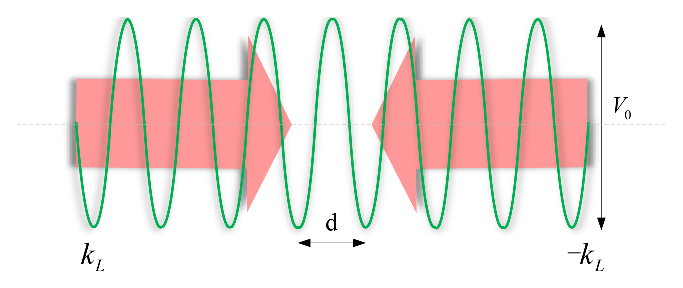
\includegraphics[width = 6cm]{fig1.eps}
  \caption{\label{fig1} The optical lattice is produced by a pair of laser beams.The two laser beams propagate in the opposite direction form a standing wave field. 
  This force is periodic. The corresponding periodic optical potential well is obtained.}
\end{figure}
The potential function of one-dimensional optical lattice is as follows:
\begin{equation}
  V=\frac{V_{0}}{2} \cos (2 k x)
  \label{eq1}
\end{equation}
However, when the two lasers do not have exactly the same parameter(for example, there is a difference between two lasers on frequency or phase), 
the form of the potential function will change. The standing wave will move(or shaking), so the system needs to be rederived.
We call the system shaken optical lattice.
Shaken optical lattice can simulate quantum systems, its advantage is that the potential is spatiotemporal period. 
Many novel physical phenomena can be induced and deduced by spatiotemporal period in the quantum physics.
Shaken optical lattice opens up new possibilities for studying in quantum matter.\cite{clark2018observation, weidner2018experimental, zhang2017manipulating, di2011finite}
%clark2018observation:    demonstrate a density-dependent gauge field, induced by atomic interactions, for quantum gases.
%                         the gauge field results from the synchronous coupling between the interactions and micromotion of the atoms in a modulated two-dimensional optical lattice.

%weidner2018experimental: experimentally demonstrate a shaken-lattice interfermeter. atoms are trapped in the ground Bloch state of a red-detuned optical lattice.
%                         show that it can measure the sign of an applied signal and optimize the interferometer in the presence of a bias signal.

%zhang2017manipulating:   summarize current experimental methods of creating synthetic gauge fields, including Raman scheme, shaken lattices and raman dressed lattices.
%                         then discuss how synthetic gauge fields bring new physics to non-interacting system and also interacting systems.

%di2011finite:            consider ultracold bosons in a two-dimensional square optical lattice described by the Bose-Hubbard model.
%                         in addtional, an external time-dependent sinusoidal force is applied to the system, which shakes the lattice along one of the diagonals.
%                         necessary to account for higher-order-hopping terms, which are renormalized differently by the shaking, and to introduce anisotropy into the problem.

Processing the parameters of two laser beams is also called modulation. The potential function will also change:
\begin{equation}
  V=\frac{V_{0}}{2} \cos \left(2 k x+X_{0}(t)\right)
  \label{eq2}
\end{equation}

Now time-dependent term in the potential function which could affect the whole optical lattice system. 
Then the Hamiltonian of the system becomes:
\begin{equation}
  H=\frac{p^{2}}{2 M}+V_{l a t}(x, t)
  \label{eq3}
\end{equation}

$V_{l a t}(x, t)$ is not only a spatial period, but also temporal period, for the convenience of later calculation. 
We need to simplify the Eqs.~\ref{eq3}. After simplification, we can get\cite{arimondo2012kilohertz}:
%arimondo2012kilohertz: shaken optical lattices potential and Hamiltonian transformation, finally get the form we used.
%                       (3. the experimental setup:shaken optical lattices)
\begin{equation}
  H^{\prime}=\frac{\left[\widetilde{\boldsymbol{p}}+M \dot{X}_{0}\right]^{2}}{2 M}+V_{l a t}(x)-\frac{1}{2} M \dot{X}_{0}^{2}
  \label{eq4}
\end{equation}
Time dependent vector potential is induced into the system of shaken optical lattice according to the above equation Eqs.~\ref{eq4}.
\begin{equation}
  A=-M \dot{X}_{0}
  \label{eq5}
\end{equation}
The vector potential can deduce a force field as the following:
\begin{equation}
  \mathbf{F}=\frac{\partial \mathbf{A}}{\partial \mathrm{t}}=-\mathrm{M} \ddot{X}_{0}
  \label{eq6}
\end{equation}

\section{The Modulation}

Different modulation methods will lead to different forms of potential functions\cite{sias2008observation, zenesini2010tunneling}.
%sias2008observation:   observed tunneling suppression and photon-assisted tunneling of Bose-Einstein condensates in an optical lattice subjected to a constant force plus a sinusoidal shaking.
%                       frequency difference bewteen the two lattice beams, the optical lattice moved formulation and dimensionless shaking parameter K0.

%zenesini2010tunneling: the shaking of the optical lattices was realized through two different schemes, modulated frequency difference and modulated phase differece. and dynamic loclization.

Here are some common modulation methods as follow.

\subsection{Frequency Modulation}
First, it is frequency modulation.
When the frequency difference between two lasers is $\Delta v=\Delta v_{\max } \sin (\omega t)$.
The actual potential field of the shaken optical lattice is
\begin{equation}
  V_{\text {lat }}=\frac{V_{0}}{2} \cos \left(2 k\left[x-\frac{\lambda \Delta v_{\max }}{2 \omega} \cos (\omega t)\right]\right)
  \label{eq11}
\end{equation}

\begin{figure}[b]
  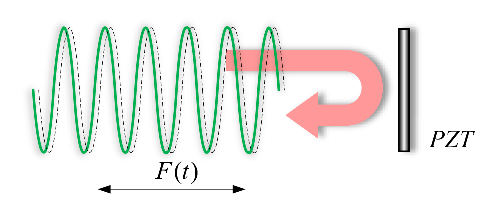
\includegraphics[width = 6cm]{fig3.eps}
  \caption{\label{fig3} Frequency modulation in thr shaken optical lattice.
  The frequency difference between the two laser beams results in the shaken optical lattice.}
\end{figure}


\subsection{Phase Modulation}
Phase modulation is another modulation method.
The system consists of a standing wave formed by the interference of the reflected light of a laser beam reflected by a plane mirror with the initial incident light. 
When the plane mirror is periodically shifted, it will change the phase of the reflected light,
so as to achieve the purpose of periodic movement of the optical lattice.

\begin{figure}[b]
  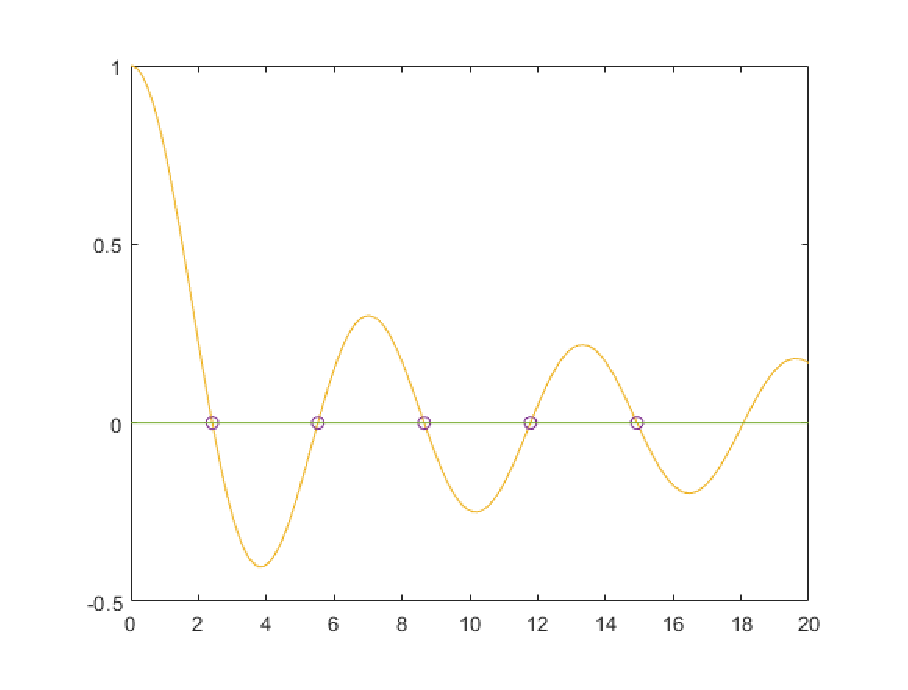
\includegraphics[width = 6cm]{fig4.eps}
  \caption{\label{fig4} The phase modulation. The phase difference between laser beam and its reflected wave emerge shaken optical lattice.}
\end{figure}

The displacement equation of plane mirror is set as $X(t)=\Delta x_{\max } \cos (\omega t)$, then the potential field in the optical lattice is
\begin{equation}
  V_{l a t}=\frac{V_{0}}{2} \cos \left(2 k\left[x-\Delta x_{\max } \cos (\omega t)\right]\right)
\end{equation}

% \subsection{Hybrid Modulation}

\section{Dynamic Localization}

In the case of tight binding approximation of single particle model, 
the corresponding time-dependent Schrodinger equation is given by the so-called Houston State.
These states give the time-dependent quasi momentum relations as follows
\begin{equation}
  q(t)=-\frac{F_{0}}{\hbar \omega} \cos (\omega t)
  \label{eq7}
\end{equation}
According to the relation of the lowest energy level in the tight binding approximation, we can get
\begin{equation}
  E^{(0)}(q)=-2 J_{0} \cos (d q)
\end{equation}
We can get the equivalent energy band relation under tight binding approximation by taking the above relation into and taking the time average in a period.
\begin{equation}
  E_{e f f}(q)=\frac{1}{T} \int_{0}^{T} d t E^{(0)}(q(t))=-2 J_{e f f} \cos (d q)
\end{equation}
Where $J_{e f f}$ is the equivalent transition matrix element, 
which is obtained by rescaling the normal transition matrix element through the zero order Bessel function in the Fig.~\ref{fig2}
\begin{figure}[b]
  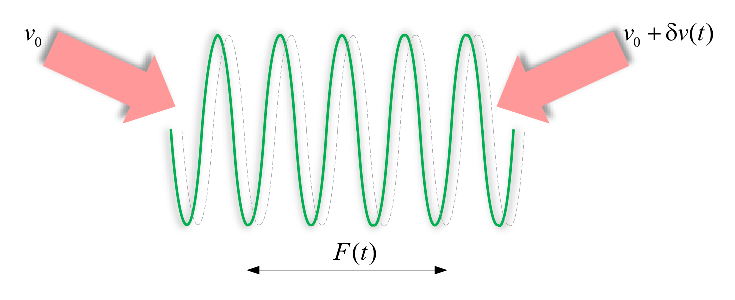
\includegraphics[width = 6cm]{fig2.eps}
  \caption{\label{fig2} Zero order Bessel function.The positions of zero points of Zero order Bessel function}
\end{figure}
\begin{equation}
  J_{e f f}=J_{0} \mathcal{J}_{0}\left(\frac{d F_{0}}{\hbar \omega}\right)=J_{0} \mathcal{J}_{0}\left(K_{0}\right)
\end{equation}
$K_{0}$ is a dimensionless parameter, which describes the intensity of modulation mode.

% \subsection{Modulation}
%frequency
From the Eqs.~\ref{eq11}, we can get the modulation intensity
\begin{equation}
  K_{0}=\frac{\mathrm{F}_{0} d}{\hbar \omega}=\frac{M d^{2} \omega \Delta v_{\max }}{\hbar \omega}=\frac{\pi^{2}}{2} \cdot \frac{\Delta v_{\max }}{\omega_{r e c}}
\end{equation}
where $\omega_{r e c}=\frac{E_{r e c}}{\hbar}$ is recoil frequency.
From the above formula, we can see the relationship between frequency modulation mode and modulation intensity. 
The modulation intensity $K_{0}$ is directly proportional to the amplitude of frequency modulation and inversely proportional to the recoil frequency. 
It is not related to the frequency of modulation. 
Of course, the recoil frequency is related to the selected cold atoms. Once selected, it will not change.
For example, $^{87} R b$ its recoil frequency is $3.24 k \times 2\pi Hz$. The relationship between modulation intensity and frequency modulation amplitude can be analyzed.
As Fig.~\ref{fig5}.

\begin{figure}[b]
  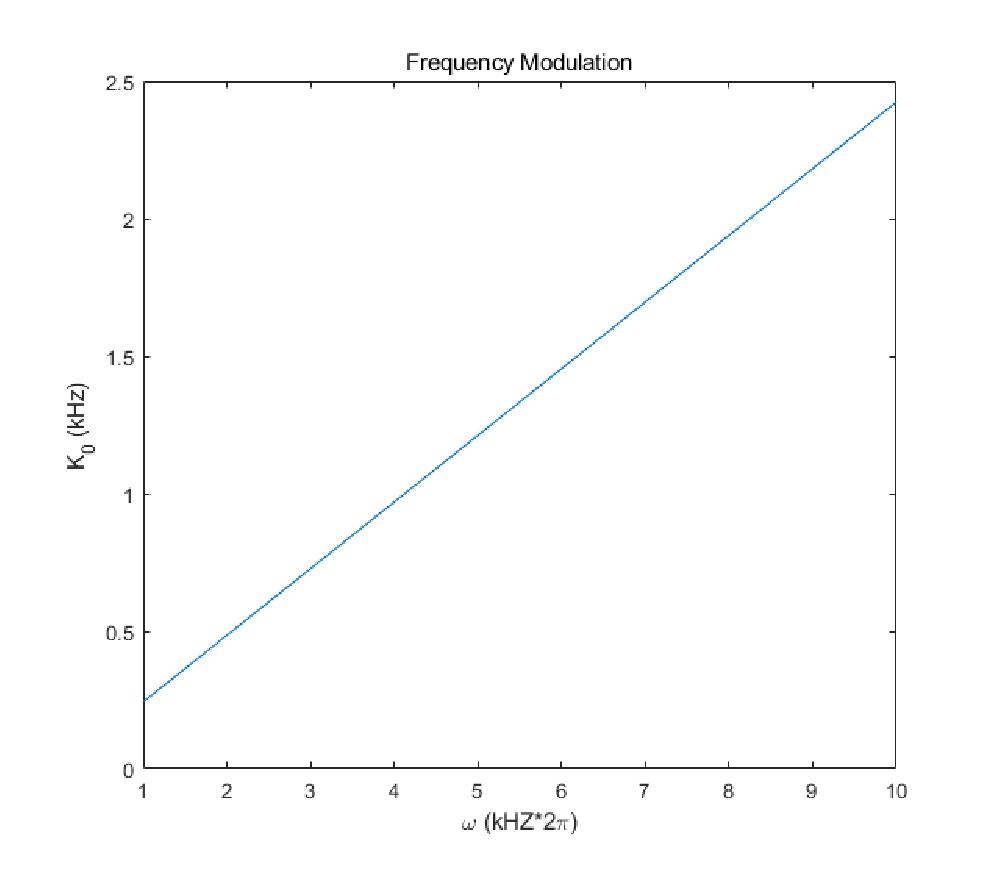
\includegraphics[width = 6cm]{fig5.eps}
  \caption{\label{fig5} The relationship between frequency modulation amplitude and modulation intensity}
\end{figure}

%phase
In this modulation mode, the modulation intensity is
\begin{equation}
  K_{0}=\frac{\mathrm{F}_{0} d}{\hbar \omega}=\frac{M \omega^{2} \omega \Delta x_{\max } d}{\hbar \omega}=\frac{\pi^{2}}{2} \frac{\omega}{\omega_{r e c}} \frac{\Delta x_{\max }}{d}
\end{equation}
The modulation intensity is related to modulation frequency, modulation amplitude, recoil frequency and lattice constant. 
Similarly, the recoil frequency and lattice constant are related to the constructed shaken optical lattice system. 
In this way, we analyze the relationship between modulation intensity and modulation frequency.

% \section{High-order Sideband generation}

% \section{Conclusion}


% \begin{figure}[b]
%   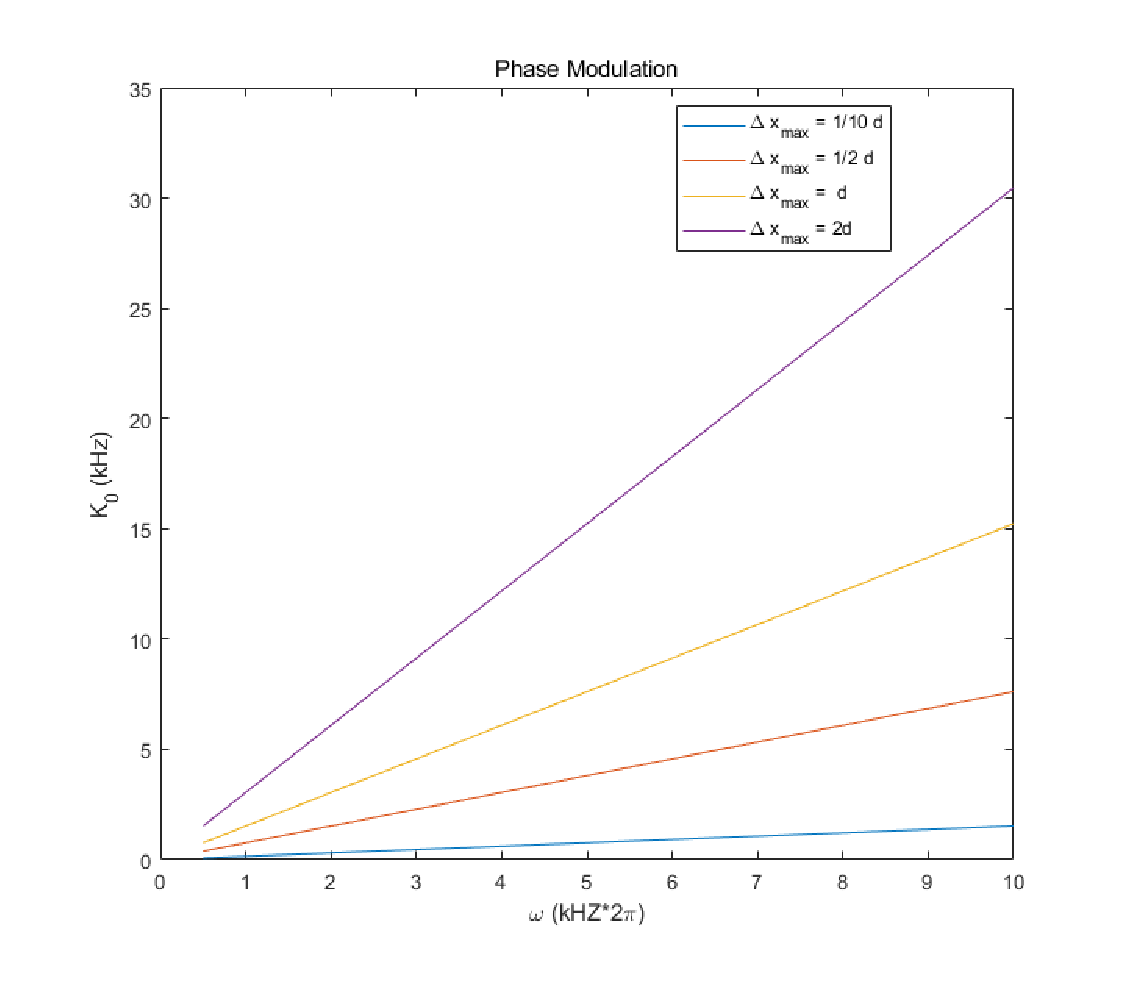
\includegraphics[width = 6cm]{fig6.eps}
%   \caption{\label{fig6} figure6}
% \end{figure}

% \begin{figure}[b]
%   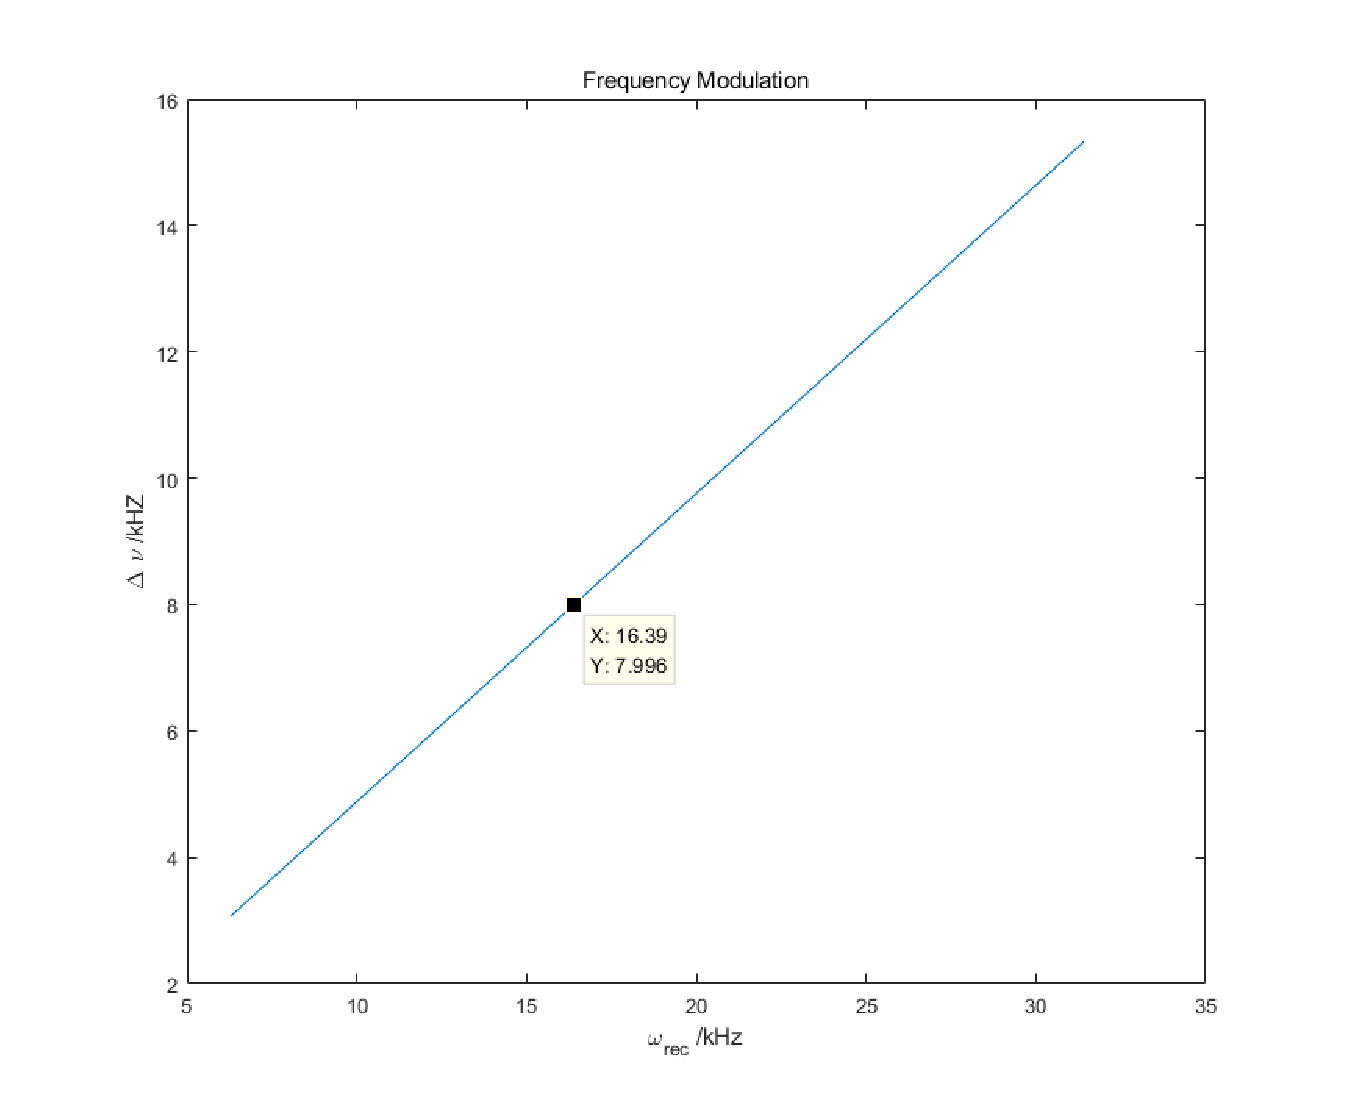
\includegraphics[width = 6cm]{fig7.eps}
%   \caption{\label{fig7} figure7}
% \end{figure}

% \begin{figure}[b]
%   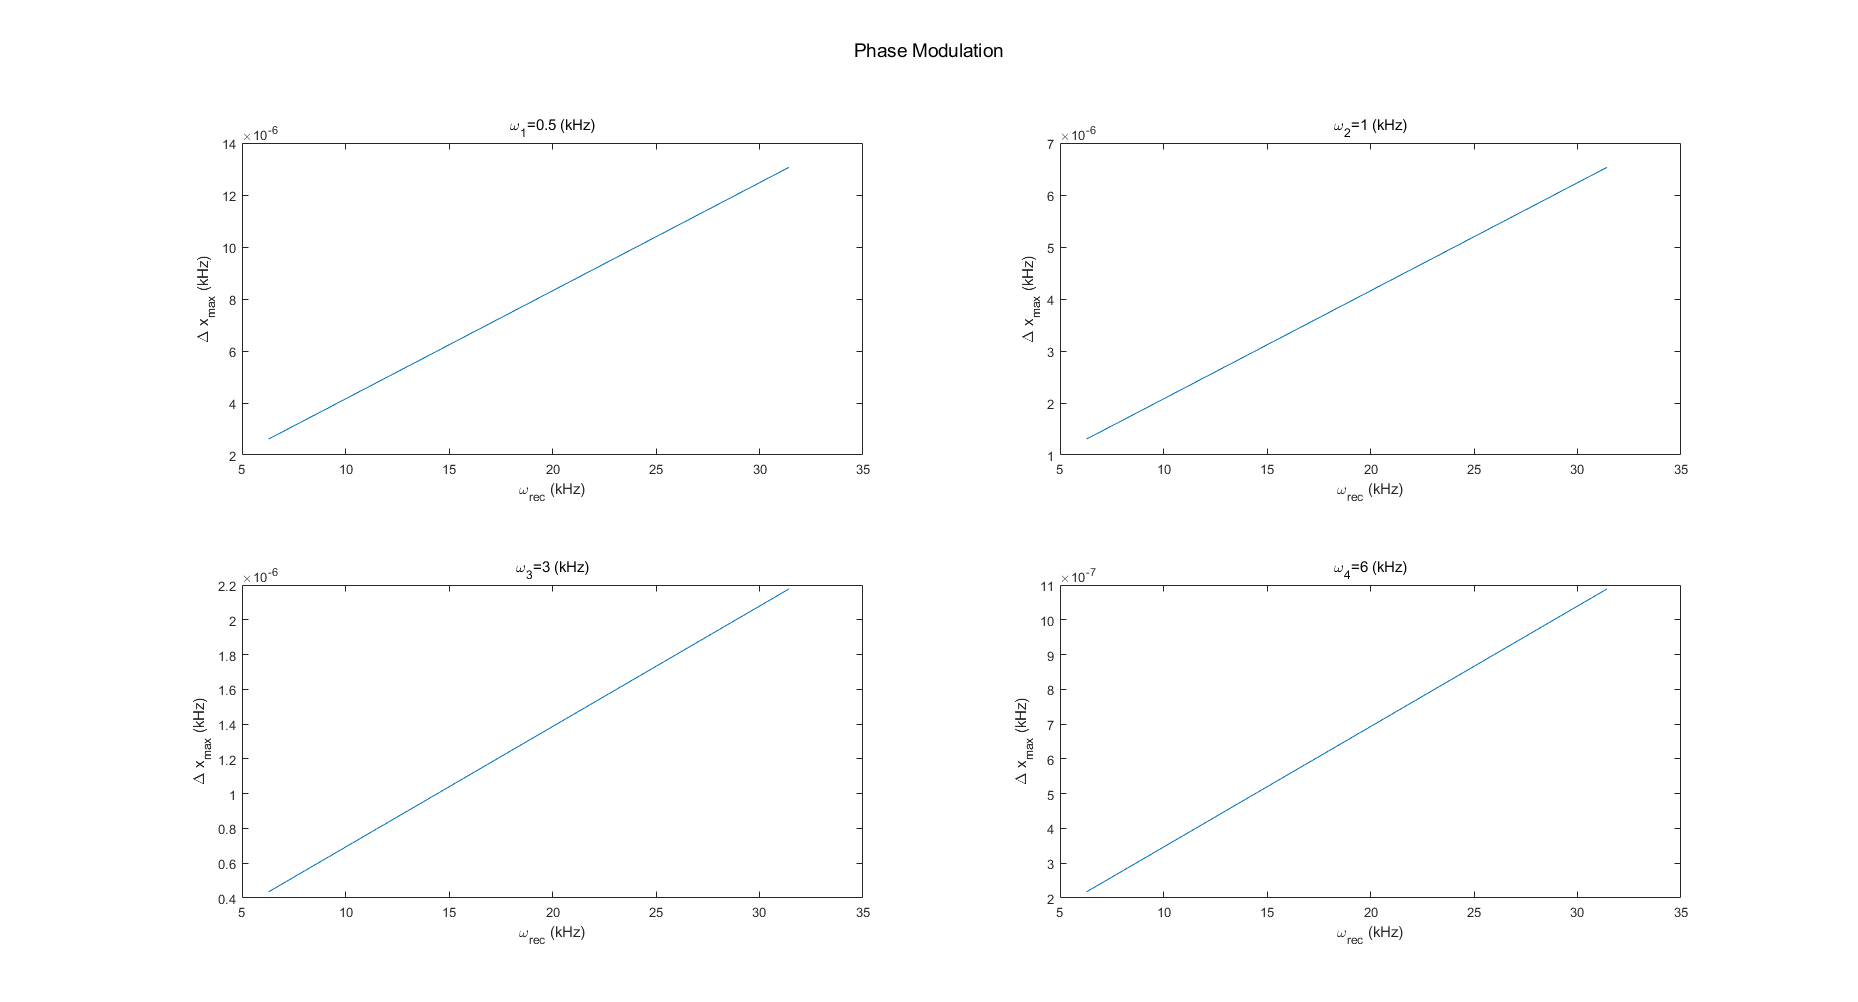
\includegraphics[width = 6cm]{fig8.eps}
%   \caption{\label{fig8} figure8}
% \end{figure}


% \begin{acknowledgments}

% \end{acknowledgments}

% \appendix


% The \nocite command causes all entries in a bibliography to be printed out
% whether or not they are actually referenced in the text. This is appropriate
% for the sample file to show the different styles of references, but authors
% most likely will not want to use it.
\nocite{*}

%\bibliography{paper}% Produces the bibliography via BibTeX.

%apsrev4-2.bst 2019-01-14 (MD) hand-edited version of apsrev4-1.bst
%Control: key (0)
%Control: author (8) initials jnrlst
%Control: editor formatted (1) identically to author
%Control: production of article title (0) allowed
%Control: page (0) single
%Control: year (1) truncated
%Control: production of eprint (0) enabled

\providecommand{\noopsort}[1]{}\providecommand{\singleletter}[1]{#1}%
\begin{thebibliography}{28}%
\makeatletter
\providecommand \@ifxundefined [1]{%
 \@ifx{#1\undefined}
}%
\providecommand \@ifnum [1]{%
 \ifnum #1\expandafter \@firstoftwo
 \else \expandafter \@secondoftwo
 \fi
}%
\providecommand \@ifx [1]{%
 \ifx #1\expandafter \@firstoftwo
 \else \expandafter \@secondoftwo
 \fi
}%
\providecommand \natexlab [1]{#1}%
\providecommand \enquote  [1]{``#1''}%
\providecommand \bibnamefont  [1]{#1}%
\providecommand \bibfnamefont [1]{#1}%
\providecommand \citenamefont [1]{#1}%
\providecommand \href@noop [0]{\@secondoftwo}%
\providecommand \href [0]{\begingroup \@sanitize@url \@href}%
\providecommand \@href[1]{\@@startlink{#1}\@@href}%
\providecommand \@@href[1]{\endgroup#1\@@endlink}%
\providecommand \@sanitize@url [0]{\catcode `\\12\catcode `\$12\catcode
  `\&12\catcode `\#12\catcode `\^12\catcode `\_12\catcode `\%12\relax}%
\providecommand \@@startlink[1]{}%
\providecommand \@@endlink[0]{}%
\providecommand \url  [0]{\begingroup\@sanitize@url \@url }%
\providecommand \@url [1]{\endgroup\@href {#1}{\urlprefix }}%
\providecommand \urlprefix  [0]{URL }%
\providecommand \Eprint [0]{\href }%
\providecommand \doibase [0]{https://doi.org/}%
\providecommand \selectlanguage [0]{\@gobble}%
\providecommand \bibinfo  [0]{\@secondoftwo}%
\providecommand \bibfield  [0]{\@secondoftwo}%
\providecommand \translation [1]{[#1]}%
\providecommand \BibitemOpen [0]{}%
\providecommand \bibitemStop [0]{}%
\providecommand \bibitemNoStop [0]{.\EOS\space}%
\providecommand \EOS [0]{\spacefactor3000\relax}%
\providecommand \BibitemShut  [1]{\csname bibitem#1\endcsname}%
\let\auto@bib@innerbib\@empty
%</preamble>
\bibitem [{\citenamefont {Jaksch}\ and\ \citenamefont
  {Zoller}(2005)}]{jaksch2005cold}%
  \BibitemOpen
  \bibfield  {author} {\bibinfo {author} {\bibfnamefont {D.}~\bibnamefont
  {Jaksch}}\ and\ \bibinfo {author} {\bibfnamefont {P.}~\bibnamefont
  {Zoller}},\ }\bibfield  {title} {\bibinfo {title} {The cold atom hubbard
  toolbox},\ }\href@noop {} {\bibfield  {journal} {\bibinfo  {journal} {Annals
  of Physics (New York)}\ }\textbf {\bibinfo {volume} {315}},\ \bibinfo {pages}
  {52} (\bibinfo {year} {2005})}\BibitemShut {NoStop}%

\bibitem [{\citenamefont {Bloch}(2005)}]{bloch2005ultracold}%
  \BibitemOpen
  \bibfield  {author} {\bibinfo {author} {\bibfnamefont {I.}~\bibnamefont
  {Bloch}},\ }\bibfield  {title} {\bibinfo {title} {Ultracold quantum gases in
  optical lattices},\ }\href@noop {} {\bibfield  {journal} {\bibinfo  {journal}
  {Nature physics}\ }\textbf {\bibinfo {volume} {1}},\ \bibinfo {pages} {23}
  (\bibinfo {year} {2005})}\BibitemShut {NoStop}%

\bibitem [{\citenamefont {Lewenstein}\ \emph {et~al.}(2007)\citenamefont
  {Lewenstein}, \citenamefont {Sanpera}, \citenamefont {Ahufinger},
  \citenamefont {Damski}, \citenamefont {Sen},\ and\ \citenamefont
  {Sen}}]{lewenstein2007ultracold}%
  \BibitemOpen
  \bibfield  {author} {\bibinfo {author} {\bibfnamefont {M.}~\bibnamefont
  {Lewenstein}}, \bibinfo {author} {\bibfnamefont {A.}~\bibnamefont {Sanpera}},
  \bibinfo {author} {\bibfnamefont {V.}~\bibnamefont {Ahufinger}}, \bibinfo
  {author} {\bibfnamefont {B.}~\bibnamefont {Damski}}, \bibinfo {author}
  {\bibfnamefont {A.}~\bibnamefont {Sen}},\ and\ \bibinfo {author}
  {\bibfnamefont {U.}~\bibnamefont {Sen}},\ }\bibfield  {title} {\bibinfo
  {title} {Ultracold atomic gases in optical lattices: mimicking condensed
  matter physics and beyond},\ }\href@noop {} {\bibfield  {journal} {\bibinfo
  {journal} {Advances in Physics}\ }\textbf {\bibinfo {volume} {56}},\ \bibinfo
  {pages} {243} (\bibinfo {year} {2007})}\BibitemShut {NoStop}%

\bibitem [{\citenamefont {Morsch}\ and\ \citenamefont
  {Oberthaler}(2006)}]{morsch2006dynamics}%
  \BibitemOpen
  \bibfield  {author} {\bibinfo {author} {\bibfnamefont {O.}~\bibnamefont
  {Morsch}}\ and\ \bibinfo {author} {\bibfnamefont {M.}~\bibnamefont
  {Oberthaler}},\ }\bibfield  {title} {\bibinfo {title} {Dynamics of
  bose-einstein condensates in optical lattices},\ }\href@noop {} {\bibfield
  {journal} {\bibinfo  {journal} {Reviews of modern physics}\ }\textbf
  {\bibinfo {volume} {78}},\ \bibinfo {pages} {179} (\bibinfo {year}
  {2006})}\BibitemShut {NoStop}%

\bibitem [{\citenamefont {Damski}\ \emph {et~al.}(2003)\citenamefont {Damski},
  \citenamefont {Zakrzewski}, \citenamefont {Santos}, \citenamefont {Zoller},\
  and\ \citenamefont {Lewenstein}}]{damski2003atomic}%
  \BibitemOpen
  \bibfield  {author} {\bibinfo {author} {\bibfnamefont {B.}~\bibnamefont
  {Damski}}, \bibinfo {author} {\bibfnamefont {J.}~\bibnamefont {Zakrzewski}},
  \bibinfo {author} {\bibfnamefont {L.}~\bibnamefont {Santos}}, \bibinfo
  {author} {\bibfnamefont {P.}~\bibnamefont {Zoller}},\ and\ \bibinfo {author}
  {\bibfnamefont {M.}~\bibnamefont {Lewenstein}},\ }\bibfield  {title}
  {\bibinfo {title} {Atomic bose and anderson glasses in optical lattices},\
  }\href@noop {} {\bibfield  {journal} {\bibinfo  {journal} {Physical review
  letters}\ }\textbf {\bibinfo {volume} {91}},\ \bibinfo {pages} {080403}
  (\bibinfo {year} {2003})}\BibitemShut {NoStop}%

\bibitem [{\citenamefont {Micheli}\ \emph {et~al.}(2006)\citenamefont
  {Micheli}, \citenamefont {Brennen},\ and\ \citenamefont
  {Zoller}}]{micheli2006toolbox}%
  \BibitemOpen
  \bibfield  {author} {\bibinfo {author} {\bibfnamefont {A.}~\bibnamefont
  {Micheli}}, \bibinfo {author} {\bibfnamefont {G.}~\bibnamefont {Brennen}},\
  and\ \bibinfo {author} {\bibfnamefont {P.}~\bibnamefont {Zoller}},\
  }\bibfield  {title} {\bibinfo {title} {A toolbox for lattice-spin models with
  polar molecules},\ }\href@noop {} {\bibfield  {journal} {\bibinfo  {journal}
  {Nature Physics}\ }\textbf {\bibinfo {volume} {2}},\ \bibinfo {pages} {341}
  (\bibinfo {year} {2006})}\BibitemShut {NoStop}%

\bibitem [{\citenamefont {Wilkin}\ and\ \citenamefont
  {Gunn}(2000)}]{wilkin2000condensation}%
  \BibitemOpen
  \bibfield  {author} {\bibinfo {author} {\bibfnamefont {N.}~\bibnamefont
  {Wilkin}}\ and\ \bibinfo {author} {\bibfnamefont {J.}~\bibnamefont {Gunn}},\
  }\bibfield  {title} {\bibinfo {title} {Condensation of “composite bosons”
  in a rotating bec},\ }\href@noop {} {\bibfield  {journal} {\bibinfo
  {journal} {Physical review letters}\ }\textbf {\bibinfo {volume} {84}},\
  \bibinfo {pages} {6} (\bibinfo {year} {2000})}\BibitemShut {NoStop}%
  
\bibitem [{\citenamefont {Jaksch}\ \emph {et~al.}(1998)\citenamefont {Jaksch},
  \citenamefont {Bruder}, \citenamefont {Cirac}, \citenamefont {Gardiner},\
  and\ \citenamefont {Zoller}}]{jaksch1998cold}%
  \BibitemOpen
  \bibfield  {author} {\bibinfo {author} {\bibfnamefont {D.}~\bibnamefont
  {Jaksch}}, \bibinfo {author} {\bibfnamefont {C.}~\bibnamefont {Bruder}},
  \bibinfo {author} {\bibfnamefont {J.~I.}\ \bibnamefont {Cirac}}, \bibinfo
  {author} {\bibfnamefont {C.~W.}\ \bibnamefont {Gardiner}},\ and\ \bibinfo
  {author} {\bibfnamefont {P.}~\bibnamefont {Zoller}},\ }\bibfield  {title}
  {\bibinfo {title} {Cold bosonic atoms in optical lattices},\ }\href@noop {}
  {\bibfield  {journal} {\bibinfo  {journal} {Physical Review Letters}\
  }\textbf {\bibinfo {volume} {81}},\ \bibinfo {pages} {3108} (\bibinfo {year}
  {1998})}\BibitemShut {NoStop}%

\bibitem [{\citenamefont {Greiner}\ \emph {et~al.}(2002)\citenamefont
  {Greiner}, \citenamefont {Mandel}, \citenamefont {Esslinger}, \citenamefont
  {Hänsch},\ and\ \citenamefont {Bloch}}]{Greiner2002Quantum}%
  \BibitemOpen
  \bibfield  {author} {\bibinfo {author} {\bibfnamefont {M.}~\bibnamefont
  {Greiner}}, \bibinfo {author} {\bibfnamefont {O.}~\bibnamefont {Mandel}},
  \bibinfo {author} {\bibfnamefont {T.}~\bibnamefont {Esslinger}}, \bibinfo
  {author} {\bibfnamefont {T.~W.}\ \bibnamefont {Hänsch}},\ and\ \bibinfo
  {author} {\bibfnamefont {I.}~\bibnamefont {Bloch}},\ }\bibfield  {title}
  {\bibinfo {title} {Quantum phase transition from a superfluid to a mott
  insulator in a gas of ultracold atoms},\ }\href@noop {} {\bibfield  {journal}
  {\bibinfo  {journal} {Nature}\ }\textbf {\bibinfo {volume} {415}},\ \bibinfo
  {pages} {39} (\bibinfo {year} {2002})}\BibitemShut {NoStop}%

\bibitem [{\citenamefont {J{\"o}rdens}\ \emph {et~al.}(2008)\citenamefont
  {J{\"o}rdens}, \citenamefont {Strohmaier}, \citenamefont {G{\"u}nter},
  \citenamefont {Moritz},\ and\ \citenamefont {Esslinger}}]{jordens2008mott}%
  \BibitemOpen
  \bibfield  {author} {\bibinfo {author} {\bibfnamefont {R.}~\bibnamefont
  {J{\"o}rdens}}, \bibinfo {author} {\bibfnamefont {N.}~\bibnamefont
  {Strohmaier}}, \bibinfo {author} {\bibfnamefont {K.}~\bibnamefont
  {G{\"u}nter}}, \bibinfo {author} {\bibfnamefont {H.}~\bibnamefont {Moritz}},\
  and\ \bibinfo {author} {\bibfnamefont {T.}~\bibnamefont {Esslinger}},\
  }\bibfield  {title} {\bibinfo {title} {A mott insulator of fermionic atoms in
  an optical lattice},\ }\href@noop {} {\bibfield  {journal} {\bibinfo
  {journal} {Nature}\ }\textbf {\bibinfo {volume} {455}},\ \bibinfo {pages}
  {204} (\bibinfo {year} {2008})}\BibitemShut {NoStop}%

\bibitem [{\citenamefont {Takamoto}\ \emph {et~al.}(2005)\citenamefont
  {Takamoto}, \citenamefont {Hong}, \citenamefont {Higashi},\ and\
  \citenamefont {Katori}}]{takamoto2005optical}%
  \BibitemOpen
  \bibfield  {author} {\bibinfo {author} {\bibfnamefont {M.}~\bibnamefont
  {Takamoto}}, \bibinfo {author} {\bibfnamefont {F.-L.}\ \bibnamefont {Hong}},
  \bibinfo {author} {\bibfnamefont {R.}~\bibnamefont {Higashi}},\ and\ \bibinfo
  {author} {\bibfnamefont {H.}~\bibnamefont {Katori}},\ }\bibfield  {title}
  {\bibinfo {title} {An optical lattice clock},\ }\href@noop {} {\bibfield
  {journal} {\bibinfo  {journal} {Nature}\ }\textbf {\bibinfo {volume} {435}},\
  \bibinfo {pages} {321} (\bibinfo {year} {2005})}\BibitemShut {NoStop}%

\bibitem [{\citenamefont {Bloom}\ \emph {et~al.}(2014)\citenamefont {Bloom},
  \citenamefont {Nicholson}, \citenamefont {Williams}, \citenamefont
  {Campbell}, \citenamefont {Bishof}, \citenamefont {Zhang}, \citenamefont
  {Zhang}, \citenamefont {Bromley},\ and\ \citenamefont
  {Ye}}]{bloom2014optical}%
  \BibitemOpen
  \bibfield  {author} {\bibinfo {author} {\bibfnamefont {B.}~\bibnamefont
  {Bloom}}, \bibinfo {author} {\bibfnamefont {T.}~\bibnamefont {Nicholson}},
  \bibinfo {author} {\bibfnamefont {J.}~\bibnamefont {Williams}}, \bibinfo
  {author} {\bibfnamefont {S.}~\bibnamefont {Campbell}}, \bibinfo {author}
  {\bibfnamefont {M.}~\bibnamefont {Bishof}}, \bibinfo {author} {\bibfnamefont
  {X.}~\bibnamefont {Zhang}}, \bibinfo {author} {\bibfnamefont
  {W.}~\bibnamefont {Zhang}}, \bibinfo {author} {\bibfnamefont
  {S.}~\bibnamefont {Bromley}},\ and\ \bibinfo {author} {\bibfnamefont
  {J.}~\bibnamefont {Ye}},\ }\bibfield  {title} {\bibinfo {title} {An optical
  lattice clock with accuracy and stability at the 10- 18 level},\ }\href@noop
  {} {\bibfield  {journal} {\bibinfo  {journal} {Nature}\ }\textbf {\bibinfo
  {volume} {506}},\ \bibinfo {pages} {71} (\bibinfo {year} {2014})}\BibitemShut
  {NoStop}%

\bibitem [{\citenamefont {Eckardt}\ \emph {et~al.}(2005)\citenamefont
  {Eckardt}, \citenamefont {Weiss},\ and\ \citenamefont
  {Holthaus}}]{eckardt2005superfluid}%
  \BibitemOpen
  \bibfield  {author} {\bibinfo {author} {\bibfnamefont {A.}~\bibnamefont
  {Eckardt}}, \bibinfo {author} {\bibfnamefont {C.}~\bibnamefont {Weiss}},\
  and\ \bibinfo {author} {\bibfnamefont {M.}~\bibnamefont {Holthaus}},\
  }\bibfield  {title} {\bibinfo {title} {Superfluid-insulator transition in a
  periodically driven optical lattice},\ }\href@noop {} {\bibfield  {journal}
  {\bibinfo  {journal} {Physical review letters}\ }\textbf {\bibinfo {volume}
  {95}},\ \bibinfo {pages} {260404} (\bibinfo {year} {2005})}\BibitemShut
  {NoStop}%

\bibitem [{\citenamefont {Ha}\ \emph {et~al.}(2015)\citenamefont {Ha},
  \citenamefont {Clark}, \citenamefont {Parker}, \citenamefont {Anderson},\
  and\ \citenamefont {Chin}}]{ha2015roton}%
  \BibitemOpen
  \bibfield  {author} {\bibinfo {author} {\bibfnamefont {L.-C.}\ \bibnamefont
  {Ha}}, \bibinfo {author} {\bibfnamefont {L.~W.}\ \bibnamefont {Clark}},
  \bibinfo {author} {\bibfnamefont {C.~V.}\ \bibnamefont {Parker}}, \bibinfo
  {author} {\bibfnamefont {B.~M.}\ \bibnamefont {Anderson}},\ and\ \bibinfo
  {author} {\bibfnamefont {C.}~\bibnamefont {Chin}},\ }\bibfield  {title}
  {\bibinfo {title} {Roton-maxon excitation spectrum of bose condensates in a
  shaken optical lattice},\ }\href@noop {} {\bibfield  {journal} {\bibinfo
  {journal} {Physical review letters}\ }\textbf {\bibinfo {volume} {114}},\
  \bibinfo {pages} {055301} (\bibinfo {year} {2015})}\BibitemShut {NoStop}%

\bibitem [{\citenamefont {Kele{\c{s}}}\ \emph {et~al.}(2017)\citenamefont
  {Kele{\c{s}}}, \citenamefont {Zhao},\ and\ \citenamefont
  {Liu}}]{kelecs2017effective}%
  \BibitemOpen
  \bibfield  {author} {\bibinfo {author} {\bibfnamefont {A.}~\bibnamefont
  {Kele{\c{s}}}}, \bibinfo {author} {\bibfnamefont {E.}~\bibnamefont {Zhao}},\
  and\ \bibinfo {author} {\bibfnamefont {W.~V.}\ \bibnamefont {Liu}},\
  }\bibfield  {title} {\bibinfo {title} {Effective theory of interacting
  fermions in shaken square optical lattices},\ }\href@noop {} {\bibfield
  {journal} {\bibinfo  {journal} {Physical Review A}\ }\textbf {\bibinfo
  {volume} {95}},\ \bibinfo {pages} {063619} (\bibinfo {year}
  {2017})}\BibitemShut {NoStop}%

\bibitem [{\citenamefont {Eckardt}\ \emph {et~al.}(2009)\citenamefont
  {Eckardt}, \citenamefont {Holthaus}, \citenamefont {Lignier}, \citenamefont
  {Zenesini}, \citenamefont {Ciampini}, \citenamefont {Morsch},\ and\
  \citenamefont {Arimondo}}]{eckardt2009exploring}%
  \BibitemOpen
  \bibfield  {author} {\bibinfo {author} {\bibfnamefont {A.}~\bibnamefont
  {Eckardt}}, \bibinfo {author} {\bibfnamefont {M.}~\bibnamefont {Holthaus}},
  \bibinfo {author} {\bibfnamefont {H.}~\bibnamefont {Lignier}}, \bibinfo
  {author} {\bibfnamefont {A.}~\bibnamefont {Zenesini}}, \bibinfo {author}
  {\bibfnamefont {D.}~\bibnamefont {Ciampini}}, \bibinfo {author}
  {\bibfnamefont {O.}~\bibnamefont {Morsch}},\ and\ \bibinfo {author}
  {\bibfnamefont {E.}~\bibnamefont {Arimondo}},\ }\bibfield  {title} {\bibinfo
  {title} {Exploring dynamic localization with a bose-einstein condensate},\
  }\href@noop {} {\bibfield  {journal} {\bibinfo  {journal} {Physical Review
  A}\ }\textbf {\bibinfo {volume} {79}},\ \bibinfo {pages} {013611} (\bibinfo
  {year} {2009})}\BibitemShut {NoStop}%

\bibitem [{\citenamefont {Zheng}\ and\ \citenamefont
  {Zhai}(2014)}]{zheng2014floquet}%
  \BibitemOpen
  \bibfield  {author} {\bibinfo {author} {\bibfnamefont {W.}~\bibnamefont
  {Zheng}}\ and\ \bibinfo {author} {\bibfnamefont {H.}~\bibnamefont {Zhai}},\
  }\bibfield  {title} {\bibinfo {title} {Floquet topological states in shaking
  optical lattices},\ }\href@noop {} {\bibfield  {journal} {\bibinfo  {journal}
  {Physical Review A}\ }\textbf {\bibinfo {volume} {89}},\ \bibinfo {pages}
  {061603} (\bibinfo {year} {2014})}\BibitemShut {NoStop}%

\bibitem [{\citenamefont {Luo}\ and\ \citenamefont
  {Zhang}(2018)}]{luo2018self}%
  \BibitemOpen
  \bibfield  {author} {\bibinfo {author} {\bibfnamefont {X.-W.}\ \bibnamefont
  {Luo}}\ and\ \bibinfo {author} {\bibfnamefont {C.}~\bibnamefont {Zhang}},\
  }\bibfield  {title} {\bibinfo {title} {Self-adapted floquet dynamics of
  ultracold bosons in a cavity},\ }\href@noop {} {\bibfield  {journal}
  {\bibinfo  {journal} {Physical review letters}\ }\textbf {\bibinfo {volume}
  {120}},\ \bibinfo {pages} {263202} (\bibinfo {year} {2018})}\BibitemShut
  {NoStop}%

\bibitem [{\citenamefont {Mei}\ \emph {et~al.}(2014)\citenamefont {Mei},
  \citenamefont {You}, \citenamefont {Zhang}, \citenamefont {Yang},
  \citenamefont {Fazio}, \citenamefont {Zhu},\ and\ \citenamefont
  {Kwek}}]{mei2014topological}%
  \BibitemOpen
  \bibfield  {author} {\bibinfo {author} {\bibfnamefont {F.}~\bibnamefont
  {Mei}}, \bibinfo {author} {\bibfnamefont {J.-B.}\ \bibnamefont {You}},
  \bibinfo {author} {\bibfnamefont {D.-W.}\ \bibnamefont {Zhang}}, \bibinfo
  {author} {\bibfnamefont {X.}~\bibnamefont {Yang}}, \bibinfo {author}
  {\bibfnamefont {R.}~\bibnamefont {Fazio}}, \bibinfo {author} {\bibfnamefont
  {S.-L.}\ \bibnamefont {Zhu}},\ and\ \bibinfo {author} {\bibfnamefont {L.~C.}\
  \bibnamefont {Kwek}},\ }\bibfield  {title} {\bibinfo {title} {Topological
  insulator and particle pumping in a one-dimensional shaken optical lattice},\
  }\href@noop {} {\bibfield  {journal} {\bibinfo  {journal} {Physical Review
  A}\ }\textbf {\bibinfo {volume} {90}},\ \bibinfo {pages} {063638} (\bibinfo
  {year} {2014})}\BibitemShut {NoStop}%

\bibitem [{\citenamefont {Grushin}\ \emph {et~al.}(2014)\citenamefont
  {Grushin}, \citenamefont {G\'omez-Le\'on},\ and\ \citenamefont
  {Neupert}}]{grushin2014floquet}%
  \BibitemOpen
  \bibfield  {author} {\bibinfo {author} {\bibfnamefont {A.~G.}\ \bibnamefont
  {Grushin}}, \bibinfo {author} {\bibfnamefont {A.}~\bibnamefont
  {G\'omez-Le\'on}},\ and\ \bibinfo {author} {\bibfnamefont {T.}~\bibnamefont
  {Neupert}},\ }\bibfield  {title} {\bibinfo {title} {Floquet fractional chern
  insulators},\ }\href {https://doi.org/10.1103/PhysRevLett.112.156801}
  {\bibfield  {journal} {\bibinfo  {journal} {Phys. Rev. Lett.}\ }\textbf
  {\bibinfo {volume} {112}},\ \bibinfo {pages} {156801} (\bibinfo {year}
  {2014})}\BibitemShut {NoStop}%

\bibitem [{\citenamefont {B\'eri}\ and\ \citenamefont
  {Cooper}(2011)}]{beri2011z}%
  \BibitemOpen
  \bibfield  {author} {\bibinfo {author} {\bibfnamefont {B.}~\bibnamefont
  {B\'eri}}\ and\ \bibinfo {author} {\bibfnamefont {N.~R.}\ \bibnamefont
  {Cooper}},\ }\bibfield  {title} {\bibinfo {title} {${\mathbb{z}}_{2}$
  topological insulators in ultracold atomic gases},\ }\href
  {https://doi.org/10.1103/PhysRevLett.107.145301} {\bibfield  {journal}
  {\bibinfo  {journal} {Phys. Rev. Lett.}\ }\textbf {\bibinfo {volume} {107}},\
  \bibinfo {pages} {145301} (\bibinfo {year} {2011})}\BibitemShut {NoStop}%

\bibitem [{\citenamefont {Clark}\ \emph {et~al.}(2018)\citenamefont {Clark},
  \citenamefont {Anderson}, \citenamefont {Feng}, \citenamefont {Gaj},
  \citenamefont {Levin},\ and\ \citenamefont {Chin}}]{clark2018observation}%
  \BibitemOpen
  \bibfield  {author} {\bibinfo {author} {\bibfnamefont {L.~W.}\ \bibnamefont
  {Clark}}, \bibinfo {author} {\bibfnamefont {B.~M.}\ \bibnamefont {Anderson}},
  \bibinfo {author} {\bibfnamefont {L.}~\bibnamefont {Feng}}, \bibinfo {author}
  {\bibfnamefont {A.}~\bibnamefont {Gaj}}, \bibinfo {author} {\bibfnamefont
  {K.}~\bibnamefont {Levin}},\ and\ \bibinfo {author} {\bibfnamefont
  {C.}~\bibnamefont {Chin}},\ }\bibfield  {title} {\bibinfo {title}
  {Observation of density-dependent gauge fields in a bose-einstein condensate
  based on micromotion control in a shaken two-dimensional lattice},\
  }\href@noop {} {\bibfield  {journal} {\bibinfo  {journal} {Physical review
  letters}\ }\textbf {\bibinfo {volume} {121}},\ \bibinfo {pages} {030402}
  (\bibinfo {year} {2018})}\BibitemShut {NoStop}%

\bibitem [{\citenamefont {Weidner}\ and\ \citenamefont
  {Anderson}(2018)}]{weidner2018experimental}%
  \BibitemOpen
  \bibfield  {author} {\bibinfo {author} {\bibfnamefont {C.}~\bibnamefont
  {Weidner}}\ and\ \bibinfo {author} {\bibfnamefont {D.~Z.}\ \bibnamefont
  {Anderson}},\ }\bibfield  {title} {\bibinfo {title} {Experimental
  demonstration of shaken-lattice interferometry},\ }\href@noop {} {\bibfield
  {journal} {\bibinfo  {journal} {Physical review letters}\ }\textbf {\bibinfo
  {volume} {120}},\ \bibinfo {pages} {263201} (\bibinfo {year}
  {2018})}\BibitemShut {NoStop}%

\bibitem [{\citenamefont {Zhang}\ and\ \citenamefont
  {Zhou}(2017)}]{zhang2017manipulating}%
  \BibitemOpen
  \bibfield  {author} {\bibinfo {author} {\bibfnamefont {S.-L.}\ \bibnamefont
  {Zhang}}\ and\ \bibinfo {author} {\bibfnamefont {Q.}~\bibnamefont {Zhou}},\
  }\bibfield  {title} {\bibinfo {title} {Manipulating novel quantum phenomena
  using synthetic gauge fields},\ }\href@noop {} {\bibfield  {journal}
  {\bibinfo  {journal} {Journal of Physics B: Atomic, Molecular and Optical
  Physics}\ }\textbf {\bibinfo {volume} {50}},\ \bibinfo {pages} {222001}
  (\bibinfo {year} {2017})}\BibitemShut {NoStop}%

\bibitem [{\citenamefont {Di~Liberto}\ \emph {et~al.}(2011)\citenamefont
  {Di~Liberto}, \citenamefont {Tieleman}, \citenamefont {Branchina},\ and\
  \citenamefont {Smith}}]{di2011finite}%
  \BibitemOpen
  \bibfield  {author} {\bibinfo {author} {\bibfnamefont {M.}~\bibnamefont
  {Di~Liberto}}, \bibinfo {author} {\bibfnamefont {O.}~\bibnamefont
  {Tieleman}}, \bibinfo {author} {\bibfnamefont {V.}~\bibnamefont
  {Branchina}},\ and\ \bibinfo {author} {\bibfnamefont {C.~M.}\ \bibnamefont
  {Smith}},\ }\bibfield  {title} {\bibinfo {title} {Finite-momentum
  bose-einstein condensates in shaken two-dimensional square optical
  lattices},\ }\href@noop {} {\bibfield  {journal} {\bibinfo  {journal}
  {Physical Review A}\ }\textbf {\bibinfo {volume} {84}},\ \bibinfo {pages}
  {013607} (\bibinfo {year} {2011})}\BibitemShut {NoStop}%

\bibitem [{\citenamefont {Arimondo}\ \emph {et~al.}(2012)\citenamefont
  {Arimondo}, \citenamefont {Ciampini}, \citenamefont {Eckardt}, \citenamefont
  {Holthaus},\ and\ \citenamefont {Morsch}}]{arimondo2012kilohertz}%
  \BibitemOpen
  \bibfield  {author} {\bibinfo {author} {\bibfnamefont {E.}~\bibnamefont
  {Arimondo}}, \bibinfo {author} {\bibfnamefont {D.}~\bibnamefont {Ciampini}},
  \bibinfo {author} {\bibfnamefont {A.}~\bibnamefont {Eckardt}}, \bibinfo
  {author} {\bibfnamefont {M.}~\bibnamefont {Holthaus}},\ and\ \bibinfo
  {author} {\bibfnamefont {O.}~\bibnamefont {Morsch}},\ }\bibfield  {title}
  {\bibinfo {title} {Kilohertz-driven bose--einstein condensates in optical
  lattices},\ }in\ \href@noop {} {\emph {\bibinfo {booktitle} {Advances in
  Atomic, Molecular, and Optical Physics}}},\ Vol.~\bibinfo {volume} {61}\
  (\bibinfo  {publisher} {Elsevier},\ \bibinfo {year} {2012})\ pp.\ \bibinfo
  {pages} {515--547}\BibitemShut {NoStop}%

\bibitem [{\citenamefont {Sias}\ \emph {et~al.}(2008)\citenamefont {Sias},
  \citenamefont {Lignier}, \citenamefont {Singh}, \citenamefont {Zenesini},
  \citenamefont {Ciampini}, \citenamefont {Morsch},\ and\ \citenamefont
  {Arimondo}}]{sias2008observation}%
  \BibitemOpen
  \bibfield  {author} {\bibinfo {author} {\bibfnamefont {C.}~\bibnamefont
  {Sias}}, \bibinfo {author} {\bibfnamefont {H.}~\bibnamefont {Lignier}},
  \bibinfo {author} {\bibfnamefont {Y.}~\bibnamefont {Singh}}, \bibinfo
  {author} {\bibfnamefont {A.}~\bibnamefont {Zenesini}}, \bibinfo {author}
  {\bibfnamefont {D.}~\bibnamefont {Ciampini}}, \bibinfo {author}
  {\bibfnamefont {O.}~\bibnamefont {Morsch}},\ and\ \bibinfo {author}
  {\bibfnamefont {E.}~\bibnamefont {Arimondo}},\ }\bibfield  {title} {\bibinfo
  {title} {Observation of photon-assisted tunneling in optical lattices},\
  }\href@noop {} {\bibfield  {journal} {\bibinfo  {journal} {Physical review
  letters}\ }\textbf {\bibinfo {volume} {100}},\ \bibinfo {pages} {040404}
  (\bibinfo {year} {2008})}\BibitemShut {NoStop}%
  
\bibitem [{\citenamefont {Zenesini}\ \emph {et~al.}(2010)\citenamefont
  {Zenesini}, \citenamefont {Lignier}, \citenamefont {Sias}, \citenamefont
  {Morsch}, \citenamefont {Ciampini},\ and\ \citenamefont
  {Arimondo}}]{zenesini2010tunneling}%
  \BibitemOpen
  \bibfield  {author} {\bibinfo {author} {\bibfnamefont {A.}~\bibnamefont
  {Zenesini}}, \bibinfo {author} {\bibfnamefont {H.}~\bibnamefont {Lignier}},
  \bibinfo {author} {\bibfnamefont {C.}~\bibnamefont {Sias}}, \bibinfo {author}
  {\bibfnamefont {O.}~\bibnamefont {Morsch}}, \bibinfo {author} {\bibfnamefont
  {D.}~\bibnamefont {Ciampini}},\ and\ \bibinfo {author} {\bibfnamefont
  {E.}~\bibnamefont {Arimondo}},\ }\bibfield  {title} {\bibinfo {title}
  {Tunneling control and localization for bose-einstein condensates in a
  frequency modulated optical lattice},\ }\href@noop {} {\bibfield  {journal}
  {\bibinfo  {journal} {Laser physics}\ }\textbf {\bibinfo {volume} {20}},\
  \bibinfo {pages} {1182} (\bibinfo {year} {2010})}\BibitemShut {NoStop}%
\end{thebibliography}%


\end{document}
